\begin{problem}%
{Экономия на рейсах}%
{\textsl{стандартный ввод}}%
{\textsl{стандартный вывод}}%
{2 секунды}%
{256 мегабайт}{}

Как вы помните, Джонни работает в министерстве финансов одной небольшой страны. По роду службы ему приходится инспектировать отечественные авиакомпании и изучать маршруты, которые те предлагают.\\

В стране есть $n$ городов. По государственным законам авиакомпания должна предоставлять услуги двустороннего перелёта между некоторыми парами городов, причём в целях унификации и стандартизации продолжительность любого полёта должна составлять ровно один день.\\

Авиакомпания называется \textit{крупной}, если с помощью рейсов этой компании можно добраться из любого города страны до любого другого. \textit{Крупная} авиакомпания называется \textit{экономной}, если при этом количество маршрутов, ею предлагаемое, минимально возможное, которое может быть у \textit{крупной} компании.\\

Государственная антимонопольная служба возбудила расследование против \textit{крупной} авиакомпании «Aero-float». Ей предъявлено обвинение в излишней неэкономности. Джонни было поручено проинспектировать «Aero-float» в целях обнаружения финансовых махинаций, но авиакомпания отказалась раскрывать полный список предоставляемых ею прямых рейсов. После продолжительных переговоров руководство компании согласилось сообщить Джонни информацию о минимально возможном количестве перелётов между каждой парой городов, если использовать только прямые рейсы «Aero-float».\\

Используя эту информацию, помогите Джонни установить, может ли компания «Aero-float» быть \textit{экономной} или нет? Более формально, установите, существует ли набор рейсов, при котором число рейсов в кратчайших маршрутах именно такие, как было сообщено Джонни, и при котором компания является \textit{экономной}?

\InputFile

В первой строке содержится единственное целое число $n$ ($2 \le n \le 250$) — количество городов в стране.\\

Далее идёт n строк, содержащих по $n$ целых чисел $T_{i,j}$: $j$-е число в $i$-й строке равняется минимальному количеству перелётов, требуемому на перемещение из $i$-го города в $j$-й.\\

Гарантируется, что предоставленная информация корректна, то есть существует некоторый набор рейсов, который соответствует данному набору чисел $T_{i,j}$.

\OutputFile

Выведите «YES», если компания «Aerofloat» может являться \textit{экономной}, или «NO» в противном случае.

\Examples

\begin{example}
\exmp{
5
0 2 1 1 1
2 0 1 3 3
1 1 0 2 2
1 3 2 0 2
1 3 2 2 0
}{%
YES
}%
\exmp{
4
0 1 1 1
1 0 2 2
1 2 0 1
1 2 1 0
}{%
NO
}%
\end{example}

\Explanation

Для первого примера ниже приведён возможный вариант предлагаемых компанией маршрутов, при котором она является экономной. На рисунке соединены те пары городов, между которыми есть прямые рейсы.

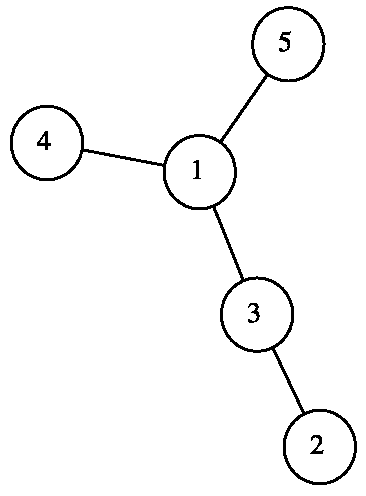
\includegraphics[scale=0.5]{images/1.png}

\end{problem}